\documentclass[14pt]{extreport}

\usepackage{gost}
\usepackage{listings}
\usepackage{longtable,rotating}
\usepackage{threeparttable}

\begin{document}

%\includepdf[pages={1}]{titul.pdf}

\newcommand\scalemath[2]{\scalebox{#1}{\mbox{\ensuremath{\displaystyle #2}}}}

% Математическое моделирование течений мелкой воды методом конечных элементов


\tableofcontents
\intro

// ОБОЗНАЧЕНИЯ И СОКРАЩЕНИЯ

Выполненная выпускная квалификационная работа посвящена задаче течения жидкости в озере, для которой требуется составить и решить систему дифференциальных уравнений с использованием метода конечных элементов (МКЭ). Предполагается, что глубина озера постоянна, а сам озеро однородно. Необходимо учесть, что озеро подвержено влиянию ветра, а так же требуется рассмотреть данную задачу с различными параметрами и проанализировать полученные результаты.

На данный момент во многих случаях не оправдывается применение более сложных математических моделей для исследования течений в прибрежных водах и озерах, чем моделей, основанных на численном решении двумерных уравнений, полученных путем применения осредненных по вертикали характеристик - уравнений мелкой воды. Трехмерные решения нецелесообразны, так как они требуют намного большего количества исходной информации и машинного времени даже с учетом современных вычислительных мощностей.

Целью представленной выпускной квалификационной работы является осуществление математического моделирования течений мелкой воды с помощью метода конечных элементов, который уже давно зарекомендовал в таких областях как механика деформируемого тела, электродинамика и конечно же гидродинамика. Данный метод является оптимальным для решения поставленной задачи так как именно он дает возможность применять достаточно гибкую разбивку рассматриваемой области и при его использовании достаточно удовлетворить лишь главным граничным условиям.

Актуальность данной работы обусловлена тем, что со второй половины 20-го века метод математического моделирования стал рабочим инструментом при изучении многих научно-технических задач, в частности, и в области гидродинамики. Основной составляющей этого метода стал является вычислительных эксперимент, широкое применение которого стало возможным благодаря развитию производительности ЭВМ и численных алгоритмов. Вычислительный эксперимент позволяет получить информацию о структуре течения при относительно небольших временных, трудовых и материальных затратах. конечно, при этом соответствующая математическая модель должна быть адекватной физическому процессу.

Научная новизна работы заключается в применении МКЭ конкретно к уравнениям мелкой воды и составлении программной реализации на языке программирования Python.

В данной работе будут представлены основные определения и понятия для уравнений мелкой воды, которые позволят составить и решить поставленную задачу, которая состоит из двух частей: аналитической и численной. Аналитически будут описаны течения жидкости при пренебрежении температурными эффектами, для которых широко используются классические уравнения Сен-Венана. После этого с помощью МКЭ будет построена и рассчитана математическая модель. Для реализации такой модели была написана программа, которая выдает результаты решения системы уравнений мелкой воды, а так же генерирует графики, которые наглядным образом отображают полученные результаты.

\chapter{Уравнения мелкой воды}

Запишем два основных уравнения для жидкости. Это уравнение количества движения и уравнение неразрывности \cite{Konor:1979:FEM}:

\begin{gather}
-\frac{\partial p}{\partial x_k} + \frac{\partial \tau_{ik}}{\partial x_i} + \rho b_k = \frac{\partial}{\partial x_i}(\rho v_i v_k) + \frac{\partial}{\partial t}(\rho v_k);
\end{gather}.

\begin{gather}
\frac{D\rho}{Dt}+\rho \frac{\partial v_i}{\partial x_i} =0
\end{gather}

Если в (1.1) и (1.2) пренебречь температурными эффектами, получим:

\begin{gather}-\frac{\partial p}{\partial x_k} + \frac{\partial \tau_{ik}}{\partial x_i} + \rho b_k = \frac{D(\rho v_k)}{Dt}
\end{gather}

\begin{gather}\frac{\partial (\rho v_i)}{\partial t} + \frac{\partial \rho}{\partial t}=0,
\end{gather}

\noindentгде $ p $ - давление, оказываемое на единицу площади поверхности воды, $ b_k $ - массовые силы, приходящиеся на единицу массы, $v_k$ - скорость частицы воды в направлении оси $x_k$, $\tau_{ik}$ - вязкостные составляющие вектора напряжения, $ \rho $ - массовая плотность воды.

В задачах циркуляции воды сложно применять данные уравнения из-за наличия свободной поверхности, изменения границ во время приливов и отливов и вследствие большого количества переменных.

Данные трудности могут быть упрощены, в результате чего получается уравнения мелкой воды. Первое упрощение состоит в том, что уравнение количества движения в проекции на ось $ x_3 $ записывается в виде:

\begin{gather}
-\frac{\partial p}{\partial x_3}=\rho g, 
\end{gather}

\noindentгде массовые силы отрицательны, поскольку действуют в направлении противоположном оси $ x_3 $. При выводе формулы (1.5) пренебрегаем всеми членами, которые характеризуют ускорение и соответствующими им напряжениям. Проинтегрируем выражение (1.5), и в результате получим:

\begin{gather}
p = \int\limits^\eta_{x_3} \rho g dx_3 = \rho g (\eta-x_3)+p_a,
\end{gather}

\noindent где $p_a$ атмосферное давление на поверхности воды
$\eta$ - возвышение свободной поверхности в соответствии с рисунком 1.1.

%\begin{figure}[H]
%\centerline{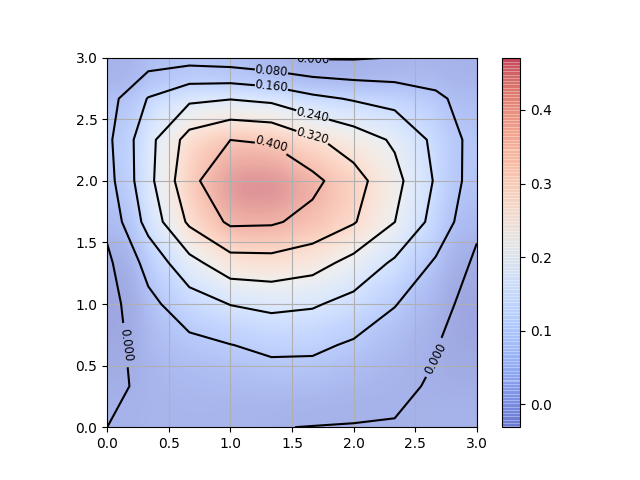
\includegraphics[width=0.5\linewidth]{1}}
%\caption{Определение типов границы}
%\label{fig11}
%\end{figure}

Оставшиеся два уравнения количества движения по направлениям $x_1$ и $x_2$ останутся без изменений:

\begin{gather}
-\frac{\partial p}{\partial x_k} + \frac{\partial \tau_{ik}}{\partial x_i} + \rho b_k = \frac{D(\rho v_k)}{Dt}.
\end{gather}

\noindentПри $k=1$ выражение (1.7) дает проекцию на ось $ x_1 $ , при $k=2$ - на ось $ x_2 $. В выражении (1.7) величина $v$ есть средняя скорость, $\rho$ - переменная массовая плотность и $\tau$ - сумма вязкостных и турбулентных напряжений.

Проинтегрируем выражения (1.4) и (1.7) по $ x_3 $. Для уравнения неразрывности это даст:

\begin{gather}
\int\limits^\eta_{-h} \bigg(\frac{\partial (\rho v_i)}{\partial x_i} + \frac{\partial \rho}{\partial t}\bigg) dx_3 =0,
\end{gather}

\noindentгде $h$ - это глубина измеряемая от базовой поверхности (в общем случае не горизонтальной).

Определим поток $ q_k $ количества жидкости (массу жидкости, приходящуюся на единицу длины и времени):


\begin{gather}
q_i = \int\limits^\eta_{-h} \rho v_i dx_3 = \rho \int\limits^\eta_{-h} v_i dx_3,
\end{gather}

\noindentПредполагается, что $\rho(x_1, x_2)$ не зависит от $x_3$.

При интегрировании уравнения (1.8) необходимо использовать кинематическое условие и правило Лейбница \cite{Zorich:2002:CALC} для вычисления частной производной интеграла с переменными пределами. Согласно этому правилу:


\begin{gather}
\frac{\partial}{\partial x_1} \int\limits^{h_2(x_1,x_2)}_{h_1(x_1,x_2)} f(x_1, x_2, x_3) dx_3=\int\limits^{h_2(x_1,x_2)}_{h_1(x_1,x_2)} \frac{\partial f}{\partial x_1} dx_3 + f \bigg|_{h_2}  \frac{\partial h_2}{\partial x_1} + f \bigg|_{h_1} \frac{\partial h_2}{\partial x_1};
\end{gather}

\noindent(аналогично для производной по $x_2$).

Кинематическое соотношение для свободной поверхности можно записать как:

\begin{gather}
v_3\bigg|_{x_2=\eta} = \frac{D\eta}{Dt} = \frac{\partial \eta}{\partial t} + v_1 \bigg|_{\eta} \frac{\partial \eta}{\partial x_1} + v_2 \bigg|_{\eta}\frac{\partial \eta}{\partial x_2}
\end{gather}

Применим формулы (1.9)-(1.11) к уравнению (1.8), и получим:

\begin{gather}
\frac{ \partial q_i}{\partial x_i} + \frac{\partial(\rho H)}{\partial t} = 0,
\end{gather}

\noindentгде $H=\eta+h $.

Чтобы проинтегрировать уравнение количества движения (1.7) по $x_3$, определим мгновенные скорости $v_1$, $v_2$:

\begin{gather}
v_1 = \overline{v_1} (x_1, x_2, t) + v_1'(x_1, x_2, x_3, t); \nonumber\\
v_2 = \overline{v_2} (x_1, x_2, t) + v_2'(x_1, x_2, x_3, t), \end{gather}

\noindentгде величина $\overline{v}$ означает средние по вертикали скорости, а $v’$ - отклонение от этих средних значений при различных значениях $x_3$.

Следовательно:

\begin{gather}
<v_k>=\int\limits^\eta_{-h} v_k dx_3 = \frac{1}{\rho} q_k, \; v_k=\frac{1}{H}<v_k>,
\end{gather}

\noindentТак как $ <v_k’> = 0 $, где знак $ <> $ означает среднее значение стоящий внутри величины.

Будем предполагать, что массовые силы обусловлены только эффектом Кориолиса. Таким образом:

\begin{gather}
b_1 = \rho f v_2, \; b_2 = - \rho f v_1.
\end{gather}
\noindentПредположим, что наклоны поверхности и дна малы по сравнению с единицей, тогда составляющие внутреннего напряжения можно аппроксимировать следующим образом:

\begin{gather}
 \tau_1\bigg|_s \approx \bigg\{ -\tau_{11}\frac{\partial \theta}{\partial x_1} -\tau_{12}\frac{\partial \theta}{\partial x_2} +\tau_{13}\bigg\}, \nonumber \\
\tau_1\bigg|_b \approx \bigg\{ \tau_{11}\frac{\partial h}{\partial x_1} +\tau_{12}\frac{\partial h}{\partial x_2} -\tau_{13}\bigg\},
\end{gather}

\noindentАналогичные значения можно выписать для величин $\tau_2|_s$ и $\tau_2|_b$.

Величины $\tau_2|_s$ и $\tau_2|_b$ можно интерпретировать как компоненты внешней силы, приложенные к поверхности и ко дну.

Подставим теперь соотношения (1.13) - (1.15) в уравнение количества движения, проинтегрированные по $x_3$ и дополнительно используем правило Лейбница и кинематическое условие. Тогда:

\begin{gather} 
\frac{\partial q_1}{\partial t} + \frac{\partial}{\partial x_1} \bigg(\frac{q_1^2}{H}\bigg)+\frac{\partial }{\partial x_2}\bigg(\frac{q_1 q_2}{H}\bigg) = -\frac{\partial N_p}{\partial x_2} + \frac{\partial N_{11}}{\partial x_1} + \frac{\partial N_{12}}{\partial x_2} \nonumber\\+ fq_2 + p\bigg|_s \frac{\partial \eta}{\partial x_1} + \tau_1\bigg|_s+p\bigg|_b\frac{\partial h}{\partial x_1} - \tau_1\bigg|_b;  \nonumber\\
\frac{\partial q_2}{\partial t} + \frac{\partial}{\partial x_1} \bigg(\frac{q_1 q_2}{H}\bigg)+\frac{\partial }{\partial x_2}\bigg(\frac{q_2^2}{H}\bigg) = -\frac{\partial N_p}{\partial x_2} + \frac{\partial N_{22}}{\partial x_2} + \frac{\partial N_{21}}{\partial x_1} \nonumber\\+ fq_1 + p\bigg|_s \frac{\partial \eta}{\partial x_2} + \tau_2\bigg|_s+p\bigg|_b\frac{\partial h}{\partial x_2} - \tau_2\bigg|_b,
\end{gather}

\noindentгде

\begin{gather} 
N_p = <p> = \int\limits^\eta_{-h} pdx_3=\rho g \frac{H^2}{2} + Hp_a; \nonumber\\
N_{11} = <\tau_{11}>-<pv_1'v_1'>; \nonumber\\
N_{22} = <\tau_{22}>-<pv_2'v_2'>; \nonumber\\
N_{12} = <\tau_{12}>-<pv_1'v_2'>;
\end{gather}

\noindentБолее того, элементы $N_{ik}$ могут быть аппроксимированы следующими выражениями:

\begin{gather} 
N_{11} \approx 2 \varepsilon_{11}\frac{\partial q_1}{\partial x_1}; \nonumber\\
N_{22} \approx 2 \varepsilon_{22}\frac{\partial q_2}{\partial x_2}; \nonumber\\
N_{12} \approx \varepsilon_{12}\bigg(\frac{\partial q_2}{\partial x_1}+\frac{\partial q_1}{\partial x_2}\bigg);
\end{gather}


\noindentгде $\varepsilon_{ik}$ обобщенные коэффициенты вихревой вязкости. Для изотропного характера течения $\varepsilon_{11}=\varepsilon_{22}=\varepsilon_{12}=\varepsilon.$

Касательные напряжения на дне обычно определяются соотношениями:

\begin{gather}
\tau_1\bigg|_b = \frac{g}{c^2} \frac{1}{\rho} \frac{q_1\sqrt{(q_1^2+q_2^2)}}{H^2}; \nonumber\\
\tau_2\bigg|_b = \frac{g}{c^2} \frac{1}{\rho} \frac{q_2\sqrt{(q_1^2+q_2^2)}}{H^2};
\end{gather}

\noindentгде $g$ - ускорение силы тяжести, $с$ - коэффициент трения, $\rho$ - плотность воды. 

Составляющие напряжения трения на поверхности воды обычно обусловлены действием ветра и могут быть найдены по формулам:

\begin{gather}
\tau_1\bigg|_s=\gamma^2\rho_aW^2\cos(\Theta); \nonumber\\
\tau_2\bigg|_s=\gamma^2\rho_aW^2\sin(\Theta);
\end{gather} 

\noindentгде $\gamma^2$ - коэффициент ветрового напряжения, $\rho_a$ - плотность воздуха, $W$ - скорость ветра, $\theta$ - угол между осью $x_1$ и направлением ветра.

Уравнения (1.17) перепишем в виде:


\begin{eqnarray} 
\frac{\partial q_1}{\partial t} + \frac{\partial}{\partial x_1} \bigg(\frac{q_1^2}{H}\bigg)+\frac{\partial }{\partial x_2}\bigg(\frac{q_1 q_2}{H}\bigg) = \frac{\partial}{\partial x_1} (N_{11}-N_p) + \frac{\partial N_{12}}{\partial x_2} + B_1; \nonumber\\
\frac{\partial q_2}{\partial t} + \frac{\partial}{\partial x_1} \bigg(\frac{q_1 q_2}{H}\bigg)+\frac{\partial }{\partial x_2}\bigg(\frac{q_2^2}{H}\bigg) = \frac{\partial}{\partial x_2} (N_{22}-N_p) + \frac{\partial N_{12}}{\partial x_2} + B_2,
\end{eqnarray}

\noindentгде

\begin{eqnarray}
B_1=fq_2+\gamma^2\rho_aW^2\cos(\Theta)-\bigg(\frac{g}{c^2}\bigg)\frac{1}{\rho}\frac{q_1\sqrt{(q_1^2+q_2^2)}}{H^2} + p_a \frac{\partial H}{\partial x_1} + \rho gH\frac{\partial h}{\partial x_1}; \nonumber\\
B_2=-fq_1+\gamma^2\rho_aW^2\sin(\Theta)-\bigg(\frac{g}{c^2}\bigg)\frac{1}{\rho}\frac{q_2\sqrt{(q_1^2+q_2^2)}}{H^2} + p_a \frac{\partial H}{\partial x_2} + \rho gH\frac{\partial h}{\partial x_2}.
\end{eqnarray}



\begin{eqnarray}
- H g \rho \frac{d}{d x_{1}} h - Pa \frac{d}{d x_{1}} H - W^{2} \gamma^{2} \rho_{a} \cos{\left (\theta \right )} - f q_{2} - \frac{d}{d x_{2}} N_{12} + \frac{d}{d t} q_{1} + \frac{\partial}{\partial x_{1}}\left(\frac{q_{1}^{2}}{H}\right) +\\ \frac{\partial}{\partial x_{2}}\left(\frac{q_{1} q_{2}}{H}\right) - \frac{\partial}{\partial x_{1}}\left(N_{11} - N_{p}\right) + \frac{g q_{1} \sqrt{q_{1}^{2} + q_{2}^{2}}}{H^{2} c^{2} \rho}


\end{eqnarray}




TODO 
Для решения окончательной системы уравнений (1.22), дополненных условием (1.12) необходимо установить требуемые граничные условия. Будем считать, что граница $S$ состоит из двух частей: твердой границы $S_1$ и жидкой $S_2$, представляющей границу рассматриваемого водоема с открытым морем в соотвествии с рисунком 1.2.

%\begin{figure}[H]
%\centerline{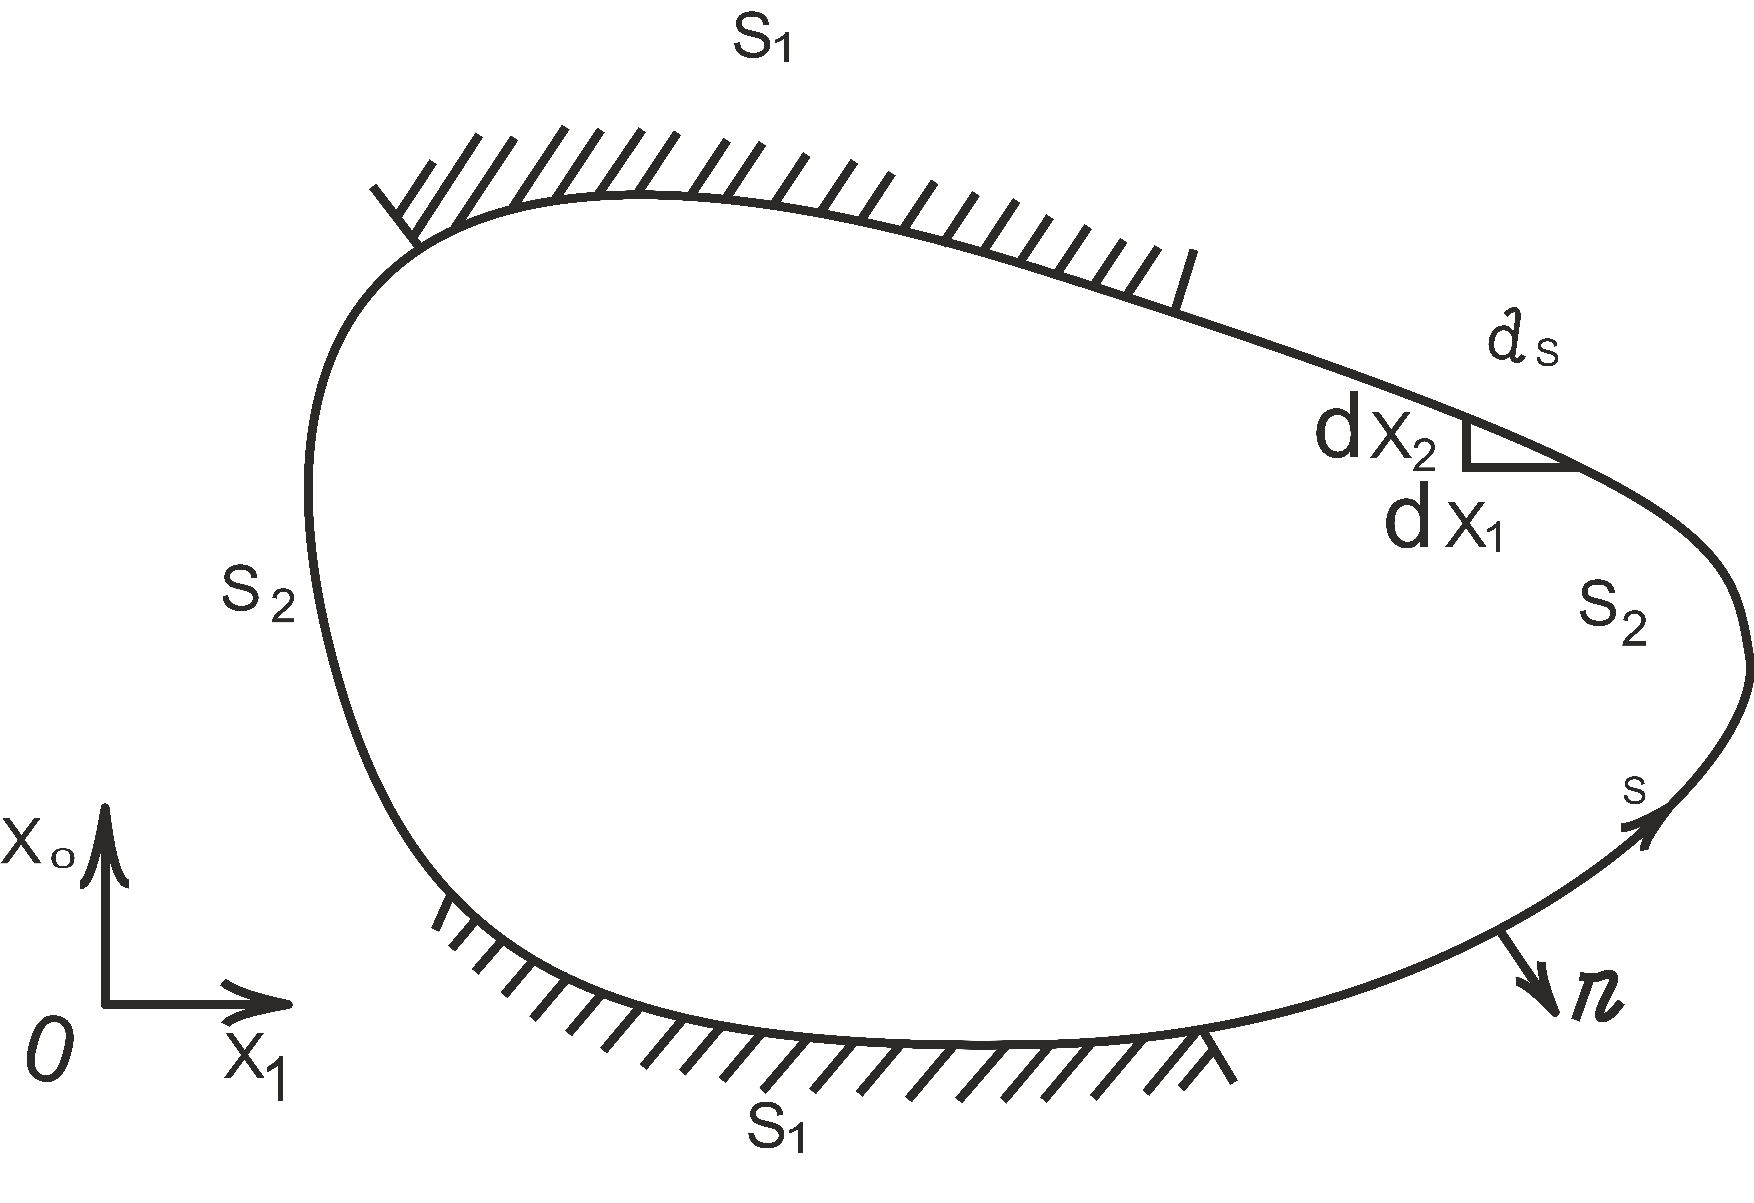
\includegraphics[width=0.5\linewidth]{2}}
%\caption{Определение типов границы}
%\label{fig11}
%\end{figure}

В системе координат $s-n$ связанной с границей течения, расход массы жидкости можно записать через $q_s$ и $q_n$:

\begin{eqnarray}
q_n=\int\limits^\eta_{-h} \rho v_n dx_3= \alpha_{n1}q_1+\alpha_{n2}q_2; \nonumber\\
q_s=\int\limits^\eta_{-h} \rho v_s dx_3= -\alpha_{n2}q_1+\alpha_{n1}q_2;
\end{eqnarray}

\noindentгде $\alpha_{n1}=\cos(\overline{n},x_1); \alpha_{n2}=\cos(\overline{n},x_2).$

Для установления результирующих сил можно воспользоваться формулами:

\begin{eqnarray}
N_{n1}=\alpha_{n1}(N_{11}-N_{p})+\alpha_{n2}N_{12}; \nonumber\\
N_{n2}=\alpha_{n1}N_{12}+\alpha_{n2}(N_{22}-N_{p}).
\end{eqnarray}

По значениями $N_{n1}$ и $N_{n2}$ определяется нормальная и касательная составляющая результирующей силы для наклонной площадки:

\begin{eqnarray}
N_{nn}=\alpha_{n1}N_{n1}+\alpha_{n2}N_{n2}; \nonumber\\
N_{ns}=\alpha_{n2}N_{n1}+\alpha_{n1}N_{n2}.
\end{eqnarray}

Если же в исследуемую акваторию впадает река, то на $ S_1 $:

\begin{eqnarray}
q_n=\overline{q_n}=|q|; \nonumber\\
q_s=0.
\end{eqnarray}

\noindentгде $|q|$ - поток втекающей
реки. 

На жидкой границе $ S_2 $ необходимо задать нормальные и касательные силы:

\begin{eqnarray}
N_{nn}=\overline{N_{nn}}; \nonumber\\
N_{ns}=\overline{N_{ns}}.
\end{eqnarray}

\noindentНо так как слагаемыми, учитывающими вихревую вязкость в уравнении (1.22) можно пренебречь, то касательные силы или скорости не могут быть заданы. Таким образом граничные условия сводятся к следующим:

\begin{eqnarray}
q_n=0 \; \text{или} \; q_n=\overline{q_n} \; \text{на} \; S_1\nonumber\\
N_{nn}=\overline{N_{nn}}=-N_p \; \text{на} \; S_2.
\end{eqnarray}


Уравнения ()-() вместе с граничными условиями () допускают вариационную формулировку и применение метода конечных элементов.

\chapter{Постановка задачи}

Пусть дана система уравнений мелкой воды, описываемая уравнениями (1.12), (1.22)-(1.23), которые были выведены в первой главе.


В качестве постоянных возьмем следующие

\begin{threeparttable}
\begin{longtable}[H]{lp{0.7\linewidth}}
$\rho$ & 1000 [кг/м\textsuperscript3] \\
$c$ & 10 [м\textsuperscript{1/2}с\textsuperscript{-1}] \\
$g$ & 9,832 [м/с\textsuperscript{2}] \\
$\gamma^2$ & 0.002 \\
$W$ & 0 [м/с] \\
$\theta$ & $0^{\circ}$ \\
$p_a$ & 100 [кПа] \\
$\rho_a$ & 1,2754 [кг/м\textsuperscript3] \\
$f$ & $0.973 \cdot 10^{-4}$ [1/с]
\end{longtable} 
\end{threeparttable}

Учитывая, что мы положили скорость ветра равную $0$, то члены $
\gamma^2\rho_aW^2\cos(\theta)$ и $
\gamma^2\rho_aW^2\sin(\theta)$ обратятся в ноль. Так же в наших уравнениях можно пренебречь членами $-fq_{1}$ и $fq_2$ так как коэффициент Кориолиса очень мал. 










Для начала данные уравнения будут переписаны в терминах методы конечных элементов, а после будет составлен алгоритм и написана программная реализация МКЭ для системы (которая выше).




\chapter{Триангуляция двумерной области}

В геометрии триангуляция дискретного множества точек $P\subset {\mathbb  {R}}^{{n+1}}$ в наиболее общем значении — это разбиение  выпуклой оболочки некого набора точек, которое представляет собой планарный граф. Одна из фигур разбиения является выпуклой оболочкой разбиваемого множества, а остальные - симплексами -  геометрическими фигурами, которые являются $n-$мерным обобщением треугольника. В любой триангуляции ($T$) формально должны выполняться следующие свойства:

	1. любые два симплекса в T пересекаются в общей грани ребра или вершины, или вообще не пересекаются;

	2. множество точек, являющихся вершинами симплексов разбиения, совпадает с множеством $P$;
	
	3. нельзя добавить ни одного нового ребра в граф без нарушения планарности.

Одно и то же множество можно триангулировать разными способами. Триангуляция дает тем лучшую аппроксимацию, чем больше её минимальный угол, при этом формируемые симплексы 'стремятся к равноугольности'. Очень важна максимизация минимального угла в вычислительных задачах, когда точность производимых вычислений очень сильно зависит от размера минимального угла триангуляции. Наилучшей в этом смысле триангуляцией является триангуляция Делоне. Простейшим способом её построения является инкрементальный алгоритм, работающий за $o(n^2)$ операций, но он не поддерживает вырожденные случаи, когда 4 точки из множества лежат на одной окружности: в этом случае триангуляция Делоне не уникальна, их несколько, но минимальные углы этих триангуляций равны. Иногда даже минимальный угол триангуляции Делоне оказывается слишком малым для устойчивой работы использующего её алгоритма, и тогда можно произвести улучшение, используя метод Руперта [J. Ruppert]. При этом будут добавлены новые вершины триангуляции, а так же образованы дополнительные треугольники. Стабильность численного алгоритма (метода конечных элементов, к примеру) может возрасти многократно за счет появления нижней границы для углов. 

\section{алгоритм Руперта [Jim Ruppert]}

Алгоритм Руперта [J. Ruppert], или же усовершенствованный алгоритм Делоне довольно новый, он был опубликован в 1994 году. Данный алгоритм адаптирован для МКЭ, а это значит, что он удовлетворяет всем требованиям, которые предъявляются к конечно-элементным сеткам, а именно:

1. треугольники не должны быть сильно вытянутыми, так как наличие таких треугольников отрицательно сказывается на точности результатов расчета;

2. должна быть учтена геометрия рассматриваемой области и в местах со сложной геометрией сетка должна сгущаться.


Если говорить точнее, алгоритм Руперта [J. Ruppert] не является алгоритмом генерации сеток. Он является лишь алгоритмом улучшения качеств сетки, от чего и произошло название. В общем случае входными данными для него будут являться геометрия конструкции в виде замкнутых полигонов и первичное разбиение конструкции на треугольники. 

При описании своего алгоритма Руперт [J. Ruppert] вводит следующую терминологию:
\begin{itemize}
\item Элемент по смыслу совпадает с конечным элементом. Это элементарная часть пространства на множество которых мы хотим разбить более сложную область этого пространства.

\item Узел — точка в которой сходятся грани и соприкасаются несколько элементов. В отличие от вершин элементов узел общий для всех соприкасающижся в одной точке элементов.

\item Сегмент — это отрезок, соединяющий две соседние точки лежащие на границе области разбиения, другими словами этот отрезок принадлежит контурам области.

\item Грань — это отрезок по которому граничат два соприкасающихся треугольника.

\item Включенная точка — любая вершина текущей сетки, которая находится внутри окружности, радиусом которой является любой сегмент.

\item "Неправильный треугольник" — треугольник неудовлетворяющий глобальным условиям, которые накладываются на генерируемую сетку.

\item Вытянутый треугольник — треугольник, имеющий одну сторону, намного отличающуюся от других двух. То есть треугольник слишком вытянут вдоль некоторой прямой. 
\end{itemize}

Алгоритм опирается на две базовые процедуры: 

\begin{enumerate}

\item Разбиение неправильного треугольника с введением нового узла

\begin{enumerate}

\item Вычисляются координаты центра окружности, описанной вокруг треугольника, подлежащего разбиению

\item В найденную точку добавляется новый узел

\item Удаляется треугольник, подлежащий разбиению и прилегающие и добавляются новые. (рис 1.)

\end{enumerate}

\item Разбиение сегмента, принадлежащего границе области разбиения с введением нового узла. 

\begin{enumerate}

\item Если в окружность, диаметром которой является сегмент, принадлежащий границе области разбиения попадает точка, не принадлежащая этому сегменту, то сегмент делится на две части;

\item Удаляется треугольник, которому принадлежал первоначальный сегмент и добавляются два новых треугольника(рис. 2).

\end{enumerate}
\end{enumerate}

\begin{figure}[H]
\centerline{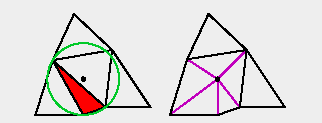
\includegraphics[width=0.5\linewidth]{figs/g2dgrid3}}
\caption{Разбиение "неправильного" треугольника
}
\label{fig11}
\end{figure}


\begin{figure}[H]
\centerline{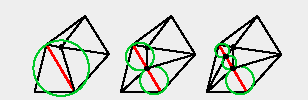
\includegraphics[width=0.5\linewidth]{figs/g2dgrid2}}
\caption{Разбиение "неправильного" сегмента посередине и добавление двух новых треугольников}
\label{fig11}
\end{figure}


Принцип работы алгоритма состоит в цикле определения 'неправильных' треугольников. В каждом треугольнике сетки определяется минимальный угол и, затем, сравниваются минимальные углы для всех треугольников с целью нахождения минимального угла сетки. Другими словами, минимальный угол в сетке равен минимально возможному углу, образованному двумя сегментами, либо двумя гранями, либо сегментом и гранью, имеющими общий узел.

Математически доказано, что критерий минимального угла автоматически обеспечивает сгущение сетки вблизи мелких подробностей: отверстий, углов и вырезов. 

Все описанные процедуры выполняются в определенной последовательности, они имеют разный приоритет. Общая схема работы алгоритма следующая:

\begin{enumerate}

\item Производится поиск включенной точки перебором всех точек и сегментов (только сегментов, но не граней).

\item Если такая точка найдена то над сегментом, который включает ее выполняется процедура деления сегмента пополам и производится возврат на шаг 1. Если включенных точек не было найдено, то алгоритм переходит на следующий шаг.

\item Производится поиск треугольника с минимальным углом.

\item Если минимальный угол меньше заданного параметра, то над треугольником, его содержащем производится процедура деления и производится возврат на шаг 1. В противном случае происходит переход на следующий шаг.

\item. Производится поиск треугольника максимальной площадью.

\item Если максимальная площадь больше заданного параметра, то над таким треугольником производится процедура деления и производится возврат на шаг 1. В противном случае происходит переход на следующий шаг.

\item Все условия удовлетворены. Конец работы алгоритма

\end{enumerate}


Автор в своей работе приводит строгие математические доказательства, гарантирующие правильную работу алгоритма при минимальном угле $\alpha < 20^{\circ}$. Данный алгоритм имеет ряд теоретических и практических преимуществ для генерации сетки.  Для не острого ввода и минимального угла порога около $20.70$ градусов алгоритм гарантированно завершает работу и создает сетку оптимального размера с постоянным коэффициентом, а так же  дает теоретически подтвержденные гарантии качества получаемой с его помощью сетки.

\section{алгоритм Чу [L. Paul Chew]}

Для МКЭ очень хорошо иметь как можно более мелкие сетки конечных элементов и в некоторых случаях, в алгоритме Руперда [J. Ruppert] получаются слишком большие сегменты. Для того, чтобы этого избежать был разработан алгоритм Чу [L. Chew], в котором сетка получается мельче за счет того, что он более консервативен в отношении разбиения на сегменты, когда граница угла меньше $30$ градусов. Главное преимущество данного алгоритма по сравнению с алгоритмом Руперда [J. Ruppert] состоит в том, что КЭ в сетке получаются с углом до $28.6$ градусов, что является несомненным плюсом, так как элементы в сетке получаются приблизительно одинаковые. Алгоритм построен на теоретической базе алгоритма Руперда [J. Ruppert], а сам алгоритм построения разбиения можно записать следующим образом:







перевести отсюда:
http://2011.cccg.ca/PDFschedule/papers/paper91.pdf





\chapter{Метод конечных элементов в двумерной области}

Метод конечных элементов \cite{Pankratov:FEM,Zenkevich:1986:FEM} - численный метод решения дифференциальных уравнений с частными производными, возникающих при решении задач прикладной физики.
	В его основе лежат две главные идеи: дискретизация исследуемого объекта и кусочно-элементная аппроксимация исследуемых функций.

Первая идея состоит в том, что область, в которой ищется решение дифференциальных уравнений, разбивается на конечное количество элементов. В каждом из элементов произвольно выбирается вид аппроксимирующей функции. Вне своего элемента аппроксимирующая функция равна нулю. Значения функций в узлах являются решением задачи и заранее неизвестны. Коэффициенты аппроксимирующих функций обычно ищутся из условия равенства значения соседних функций на границах между элементами (в узлах). Затем эти коэффициенты выражаются через значения функций в узлах элементов. Составляется система линейных алгебраических уравнений. Количество уравнений равно количеству неизвестных значений в узлах, на которых ищется решение исходной системы, прямо пропорционально количеству элементов. Так как каждый из элементов связан с ограниченным количеством соседних, система линейных алгебраических уравнений имеет разрежённый вид, что существенно упрощает её решение. 

Если говорить в матричных терминах, то собираются так называемые матрицы жёсткости и масс. Далее на эти матрицы накладываются граничные условия (например, при условиях Неймана в матрицах не меняется ничего, а при условиях Дирихле из матриц вычёркиваются строки и столбцы, соответствующие граничным узлам, так как в силу краевых условий значение соответствующих компонент решения известно). Затем собирается СЛАУ и решается.

Основное отличие МКЭ от классических алгоритмов вариационных принципов и методов невязок заключается в выборе базисных функций. Они берутся в виде кусочно-непрерывных функций, которые обращаются в ноль всюду, кроме ограниченных подобластей, являющихся конечными элементами. Это в свою очередь ведет к разреженной структуре матрицы коэффициентов разрешающей системы уравнений.

Главные достоинства МКЭ состоят в следующем:

1. исследуемые объекты могут иметь любую форму и различную физическую природу – твёрдые тела, жидкости, газы, электромагнитные среды

2. конечные элементы (КЭ) могут иметь различную криволинейную форму и различные размеры

3. можно исследовать однородные и неоднородные, изотропные и анизотропные тела с линейными и нелинейными свойствами

4. можно решать как стационарные, так и нестационарные задачи

5. можно моделировать любые граничные условия;

6. вычислительный алгоритм, представленный в матричной форме, формально единообразен для различных физических задач и для задач различной размерности. Это удобно для вычисления на ЭВМ, так как методология не меняется и фактически используется единая программа численного решения

7. на одной и той же сетке конечных элементов можно решать различные физические задачи, что облегчает анализ связанных между собой задач

8. разрешающая система уравнений имеет разреженную симметричную ленточную матрицу жёсткости, что ускоряет вычислительный процесс на ЭВМ

Перед тем как рассматривать метод конечных элементов, рассмотрим метод взвешенных невязок, который является частным случаем метода конечных элементов с одним элементом.

\section{Метод взвешенных невязок}

Рассмотрим дифференциальное уравнение вида

\begin{eqnarray}
 \mathcal A= \mathcal L\phi-p=0
\end{eqnarray}

\noindentв некоторой области $\Omega$.

Здесь $\mathcal L$ - некоторый линейный дифференциальный оператор, а $p$ не зависит от неизвестной функции $\phi$.

Решение уравнения (2.1) должно удовлетворять условию

\begin{eqnarray}
\mathcal B = \mathcal M \phi+r=0
\end{eqnarray}

\noindentНа загмнутой кривой $\Gamma$, ограничивающей область $\Omega$.

Здесь $\mathcal M$ - соотвествующий линейный дифференциальный оператор, а $r$ не зависит от неизвестной функции $\phi$.

Построим аппроксимацию для решения $\phi$, которая на граничной кривой $\Gamma$ принимает те же значения, что и $\phi$. Если найти некоторую функцию $\psi$, принимающую одинаковые с $\phi$ значения на $\Gamma$, т.е. $\psi|_\Gamma= \phi|_\Gamma$, и ввести систему линейно независимых базисных функций $\{N_m; m = 1,2, \dots, N\}$, то на $\Omega$ можно предложить следующую аппроксимацию $\hat{\phi}$ для $\phi$: 

\begin{eqnarray}
\phi \approx \hat\phi = \psi + \sum\limits_{m=1}^{M} a_mN_m,
\end{eqnarray}

\noindentгде $a_m, m= \overline{1,M}$ - некоторые параметры, вычисляемые так, чтобы получить хорошее приближение, а функция $\psi$ и базисные функции $N_m$ выбраны таким образом, что

\begin{eqnarray}
 \mathcal M\psi=-r, \; \mathcal M N_m=0, \; m=\overline{1,M} \; \text{на} \; \Gamma,
\end{eqnarray}

\noindentи поэтому $\phi$ автоматически удовлетворяет краевым условиям (2.2) при произвольных коэффициентах $a_m$. Отметим, что система базисных функций (которые также называют функциями формы) должна быть выбрана так, чтобы гарантировать улучшение аппроксимации при возрастании числа базисных функций для $M$.

Для того, чтобы найти аппроксимации производных от $\phi$, продифференцируем (2.3), получим:


\begin{gather}
\phi \approx \hat\phi = \psi + \sum\limits_{m=1}^{M} a_mN_m,\nonumber\\
\frac{\partial \phi}{\partial x} \approx \frac{\partial \hat\phi}{\partial x}=\frac{\partial \psi}{\partial x}+\sum\limits_{m=1}^{M} a_m\frac{\partial N_m}{\partial x},\nonumber\\
\frac{\partial^2 \phi}{\partial x^2} \approx \frac{\partial^2 \hat\phi}{\partial x^2}=\frac{\partial^2 \psi}{\partial x^2}+\sum\limits_{m=1}^{M} a_m\frac{\partial^2 N_m}{\partial x^2}, \nonumber
\end{gather}

\noindentи т.д.

Так как построенное разложение (2.3) удовлетворяет краевым условиям (2.2), то для получения аппроксимации искомой функции $\phi$ осталось гарантировать, что $\hat\phi$ - приближённое решение уравнения (2.1). Для этого вначале введём погрешность или невязку $R_\Omega$ в аппроксимации, определяемую по формуле


\begin{eqnarray}
R_\Omega=A(\hat\phi)=\mathcal L \hat\phi+p=\mathcal L\psi+\bigg(\sum\limits_{m=1}^{M} a_m \mathcal L N_m\bigg) +p.
\end{eqnarray}

Чтобы уменьшить эту невязку, потребуем равенства нулю соответствующего числа интегралов от погрешности \cite{Zorich:2002:CALC}, взятых с различными весами, т.е.

\begin{eqnarray}
\int_\Omega W_l R_\Omega d\Omega = \int_\Omega W_l \bigg\{\mathcal L \psi +\bigg(\sum\limits_{m=1}^{M} a_m \mathcal L N_m\bigg) +p \bigg\} d\Omega =0; \; l=\overline{1,M};
\end{eqnarray}

\noindentгде $\{W_l:l=1,2,\dots,M\}$ - это множество линейно независимых весовых (или пробных) функций.

Таким образом, система уравнений метода взвешенных невязок (2.6) сводится к системе линейных алгебраических уравнений для неизвестных коэффициентов $a_m$, которую можно записать как:

\begin{eqnarray}
Ka=f,
\end{eqnarray}

\noindentгде

\begin{gather}
a = (a_1,a_2,\dots, a_M)^T, \\
K_{lm}=\int_\Omega W_l \mathcal L N_m  d\Omega, \; l,m=\overline{1,M}; \\
f_l=-\int_\Omega W_l p d \Omega-\int_\Omega W_l \mathcal L \psi d \Omega \; l,m=\overline{1,M};
\end{gather}


\noindentВычислив элементы матрицы $K$ и столбца свободных членов $f$ и решив затем полученную систему, мы найдем $a_m,\; m=\overline{1,M}$; и тем самым закончим процесс построения приближенного решения (2.1).
\\

\section{Метод конечных элементов}
В методе взвешенных невязок предполагалось, что базисные функции $N_m$ определены одним выражением на всей области $\Omega$. При этом интегралы в аппроксимирующем уравнении (2.5) вычисляется по всей области.

С другой стороны, область $\Omega$ можно разбить на несколько непересекающихся подобластей (конечных элементов $\Omega^e$), которые могут иметь различную форму и размеры. В результате разбивки создается сетка из границ элементов:

$$\Omega=\bigcup\limits_{e=1}^E\Omega^{e}$$


\noindentПересечение границ областей $\Omega^{e}$ образуют узлы. Выбор типа и размера КЭ напрямую зависит от рассматриваемой задачи.

После того, как мы разбили рассматриваемую область $\Omega$ сеткой конечных элементов можно аппроксимировать решение уравнения отдельно для каждой подобласти $\Omega^{e}$, где базисные функции могут быть определены различным образом для каждой из подобластей. В этом случае определённые интегралы, входящие в аппроксимирующие уравнения, можно посчитать просуммировал вклады по каждому элементу:

\begin{gather}
\int_\Omega W_l R_\Omega d\Omega = \sum\limits_{e=1}^E\int_{\Omega^{e}} W_l R_\Omega d\Omega^e, \nonumber\\
\int_\Gamma \overline{W_l} R_\Gamma d\Gamma = \sum\limits_{e=1}^E\int_{\Gamma^{e}} W_l R_\Gamma d\Gamma^e;
\end{gather}


\noindentВ данных интегралах:
\begin{gather}
\sum\limits_{e=1}^E\Omega^e=\Omega, \\
\sum\limits_{e=1}^E\Gamma^e=\Gamma;
\end{gather}


\noindent где $E$ - число подобластей, на которые разбивается область $\Omega$; $\Gamma^e$ - часть границы $\Omega^e$, лежащая на $\Gamma$.

Система уравнений метода конечных элементов сводится в аналогичной системе метода взвешенных невязок (), но за исключением того, что:

\begin{gather}
	K_{lm}=\sum\limits_{e=1}^{E} K_{lm}^{e}=\sum\limits_{e=1}^{E}\int_\Omega^{e} W_l^{e} \mathcal L N_{m}^{e}  d\Omega^{e}, \; l,m=\overline{1,M}; \\
f_l=\sum\limits_{e=1}^{E} f_{l}^{e}=\sum\limits_{e=1}^{E} \bigg(-\int_{\Omeg^{e}} W_{l}^{e} p d \Omega^{e} -\int_\Omega^{e} W_{l}^{e} \mathcal L \psi d \Omega^{e}\bigg) \; l,m=\overline{1,M};
\end{gather}



Отметим так же, что для матрицы $K^{e}$ не нужно вычислять каждую компонентку, так как её компонента $K_{lm}^{e}$ равна нулю, если узлы $l$ и $m$ не принадлежат элементу $e$. 

Идея метода конечных элементов заключается в следующем: если подобласти имеют простую форму и базисные функции на этих подобластях вычисляются однотипно, то решать задачу указанным выше способом становиться очень просто. 




\section{МКЭ для рассматриваемой задачи}

$$
\phi \approx \hat\phi = \psi + \sum\limits_{m=1}^{M} a_m(t)N_m(x,y),\nonumber\\
$$

Перейдем в уравнениях (1.12), (1.22)-(1.23) к конечно-элементой формулировке. Для этого запишем $q_1, q_2, H$ через базисные функции и подставим в наши уравнения.

$q_1(x_1, x_2, t)=a_{11}(t)N_1(x_1, x_2) + a_{12}(t)N_2(x_1, x_2) + a_{13}(t)N_3(x_1, x_2)$

$q_1(x_1, x_2, t)=a_{21}(t)N_1(x_1, x_2) + a_{22}(t)N_2(x_1, x_2) + a_{23}(t)N_3(x_1, x_2)$

$H(x_1, x_2, t)=a_{31}(t)N_1(x_1, x_2) + a_{32}(t)N_2(x_1, x_2) + a_{33}(t)N_3(x_1, x_2)$


Выпишем невязку для уравнения неразрывности:

\begin{eqnarray}
R=\bigg(a_{11}(t)\frac{\partial N_1(x_1, x_2)}{\partial x_1} + a_{12}(t)\frac{\partial N_2(x_1, x_2)}{\partial x_1} + a_{13}(t)\frac{\partial N_3(x_1, x_2)}{\partial x_1} \bigg) + \\
	\bigg(a_{21}(t)\frac{\partial N_1(x_1, x_2)}{\partial x_2} + a_{22}(t)\frac{\partial N_2(x_1, x_2)}{\partial x_2} + a_{23}(t)\frac{\partial N_3(x_1, x_2)}{\partial x_2} \bigg) + \\
	\rho\bigg(\frac{d a_{31}(t)}{\partial t}N_1(x_1, x_2) + \frac{d a_{32}(t)}{\partial t}N_2(x_1, x_2) + \frac{d a_{33}(t)}{\partial t}N_3(x_1, x_2) \bigg)
\end{eqnarray}


Умножим невязку на весовую функцию и проинтегрируем по треугольнику $\Delta_e$:


\begin{eqnarray}
\bigg(a_{11}\int\limits_{\Delta_e}^{}\frac{\partial N_{e_1}}{\partial x_1}N_{m}d{\Delta_e} + \int\limits_{\Delta_e}^{}a_{12}\frac{\partial N_{e_2}}{\partial x_1}N_{m}d{\Delta_e} + \int\limits_{\Delta_e}^{}a_{13}\frac{\partial N_{e_3}}{\partial x_1}N_{m}d{\Delta_e} \bigg) + \\
	\bigg(\int\limits_{\Delta_e}^{}a_{21}\frac{\partial N_{e_1}}{\partial x_2}N_{m}d{\Delta_e} + \int\limits_{\Delta_e}^{}a_{22}\frac{\partial N_{e_2}}{\partial x_2}N_{m}d{\Delta_e} + \int\limits_{\Delta_e}^{}a_{23}\frac{\partial N_{e_3}}{\partial x_2}N_{m}d{\Delta_e} \bigg) + \\
	\rho\bigg(\dot{a_{31}}\int\limits_{\Delta_e}^{} N_{e_1}N_{m}d{\Delta_e} + \dot{a_{32}}\int\limits_{\Delta_e}^{} N_{e_2}N_{m}d{\Delta_e} + \dot{a_{33}}\int\limits_{\Delta_e}^{} N_{e_3}N_{m}d{\Delta_e}\bigg)
\end{eqnarray}



\begin{eqnarray}
\iint \left(\frac{\partial}{\partial t}\left(\rho \sum_{e=1}^{M} \operatorname{N_{k}}{\left (x_{1},x_{2} \right )} \operatorname{a_{2m+k}}{\left (t \right )}\right) + \frac{\partial}{\partial x_{1}} \sum_{e=1}^{M} \operatorname{N_{k}}{\left (x_{1},x_{2} \right )} \operatorname{a_{k}}{\left (t \right )} + \frac{\partial}{\partial x_{2}} \sum_{e=1}^{M} \operatorname{N_{k}}{\left (x_{1},x_{2} \right )} \operatorname{a_{m+k}}{\left (t \right )}\right) \operatorname{N_{l}}{\left (x_{1},x_{2} \right )}\, dx_{1}\, dx_{2}

\end{eqnarray}





\chapter{Учёт граничных условий}

тут будут учитываться граничные условия


\chapter{Изменение формы водоёма (прямоугольник, круг, реальный водоём)}

пруд - файл pond_without_islands.poly \\
пруд с островами - файл pond_with_islands.poly \\
реально озеро без острова - файл lake_svetloyar.poly



\chapter{Учёт наличия острова (островов) внутри водоёма}

реальное озеро с островами - файл - $lake_superior.poly$


\chapter{Разработка базы данных для хранения информации о проведённых экспериментах}

Тут я напишу про то, как мы будет складывать результаты в монгу.



\bibliographystyle{ugost2008}
\bibliography{biblio}


\end{document}